\documentclass[a4paper,12pt]{article}
\usepackage[english]{babel}
\author{Steven Hill}
\title{Easy Terminal Alternative}
\date{\today}


\usepackage{rotating}
\usepackage{indentfirst}
\usepackage{lineno}
\usepackage{fancyhdr}
\pagestyle{fancy}
\usepackage[utf8]{inputenc}
\usepackage{amsmath}
\usepackage{amsfonts}
\usepackage{amssymb}
\usepackage{graphicx}
\usepackage{setspace}
\usepackage{outline}
\usepackage{paralist}
\usepackage{listings}



\newcommand{\bibent}{\noindent \hangindent 40pt}
\newenvironment{workscited}{ \doublespacing \newpage \begin{center} Works Cited \end{center}}{\newpage }

\begin{document}
\maketitle
\tableofcontents

\section{Introduction}
 Easy-Terminal-Alternative (ETA) is a web driven tool for interacting with command line applications. This document contains the background and technical documentation for the Easy-Terminal-Alternative implementation at the Center for Genome Research (CGRB) and Biocomputing. ETA's primary purpose is to assist researchers with using otherwise complicated computational tools in an easy, web-driven format.
 
 The biggest flaw with ETA to date is the lack of documentation. According to Carla Schroder, author of the 
Linux cookbook, "Good documentation is equally important as good code. Sometimes there is this attitude that developer time is more valuable and important than user or potential contributor time" (Schroder). Fixing bugs in the software or implementing new features is nearly impossible in the applications current state. It is large, complex, and completely undocumented. Clearly, documentation is an important part of ETA which needs to be completed.

\subsection{Need and purpose}
 
 ETA was created in response to a need. A bottleneck in research was bridging the gap between researchers who had the ability to use the command line, and those that needed to spend time learning to use the command line. "All new tool were at the command line and it would take a great deal of time to port a tool into a web interface. This reduced the number of people who did computational work from a lack of knowledge on how to work in that environment" (Sullivan). Previously, researchers solved these problems by creating their own web portals. However, to create a new tool, developers were required to create an entirely new page. (Sullivan). It was clear there was a need for more efficient means of interfacing the command line, but there was no direction for it.
 
 Eventually, a undergraduate named Alex Boyd began development on a web portal for a tool called HAL. HAL is a pipeline for phylogenetic analyses (HAL CITELATER).
 
 "Boyd created a tool to start this process and once I talked with him about it we both realized it could be expanded into the tool we call ETA today. My [Chris Sullivan's] past knowledge of problems with programming tools onto the web and methods to interact with the cluster help drive the path we took and why the system works the way it does (wrappers, pipelines, requests)" (Sullivan). The fact that ETA was expanded on a tool originally created for one program required for it to be built with a certain amount of modularity. This modularity allowed for ETA to be expanded to work for every installed command line tool.
 
 \subsection{Goals}
When ETA was being developed, it had these goals:
 \begin{compactenum}
    \item Allow any user on the system to create new web driven forms to any command line tool in minutes/hours versus days/weeks.
    \item Take these wrappers and share them to other users and combine them together into pipelines.
 	\item Allow the computational people to focus on writing new tools
 	\item A method to upload, download and disseminate data using the interface.
 \end{compactenum}

 ETA reached these goals. The ability to create wrappers, that is, web driven forms that directly map to command line arguments, provided a solution to the first goal. With ETA, you can share all of these wrappers (stored in the MySQL database) with other researchers. To create pipelines (figure 1), users can simply drag different wrappers into the order they are to be executed. The pipeline module supports for-loops, if statements, and switch blocks as well. 
 
 Computational Scientists can now spend their time creating the best possible command line tools for researchers. To create the user interface, they can simply add a wrapper into ETA. To download or share data, you can right click on one of your files (from the CGRB filespace), and choose to download or share it. Uploading is just as easy. You can either drag the file into your browser, or click the upload button.
 
 \begin{figure}
\includegraphics[width=1\textwidth]{pipeline.png}
\caption{Screenshot of Pipeline Module}
\label{fig:pipeline}
\end{figure}


 
\section{Architecture}

ETA is built on several preexisting technologies. These technologies are, Java, Google-web-toolkit (GWT), and Apache Tomcat. Java is the programming language used for both the server application and the client application, GWT compiles java  to create the HTML and Javascript that will appear in the users browser, and Tomcat is the webserver which handles all of the requests and the application ultimately lives on.

\subsection{Aspect-Oriented Design}
In order for an application of this magnitude to be modular, it was important that the design included a way to functionally be independent of all other parts of the application. That is, if something broke on the client-side, it would not affect the other parts of the application. The primary design pattern used was an Aspect-Oriented Design. That is, an architecture that is designed around modularity. 

One study concluded that, "AO architectures tended to require less invasive changes" (Molesini et al. 722). Being able to add or modify functionality is imperative for any new technology. For example, if the Center for Genome Research and Biocomputing was to change authentication methods, ETA should be able to adapt to this new method without breaking any other parts of the application. As a result of these needs, ETA was designed with this in mind.

\subsection{Package Overview}
ETA is broken up into many different packages. "Package objects contain version information about the implementation and specification of a Java package" (Java Platform SE 7). The application is into many packages. The following is the package hierarchy:
\begin{compactenum}
    \item client:
    \begin{compactenum}
        \item button
        \item images
        \item pipeline
        \item table
        \item tabs
        \item tabset
        \item tools
        \item window
        \item wrapperrunner
    \end{compactenum}
    \item etadrive
    \begin{compactenum}
        \item desktop
    \end{compactenum}
    \item remote
    \begin{compactenum}
        \item api
    \end{compactenum}
    \item server
    \begin{compactenum}
        \item mysql
        \item remote
        \item rmi
        \item services
        \item settings
    \end{compactenum}
    \item shared
    \begin{compactenum}
        \item etatype
        \item pipeline
        \item wrapper
    \end{compactenum}
\end{compactenum}

 Each package servers a purpose and is as decoupled as possible from the other packages. Although complete decoupling is impossible, the higher level classes are written to be as independent as possible. The main coupling that occurs is in the methods that are implemented across the platform, such as client from server, and the remote class from the server. See the UML diagram for detail about the main package relations. 

Inside of each main package, there contains more packages. These are typically reserved for inheritance between similar classes. The most obvious use of this is in the client package. Many different GUI "widgets", or things a user interacts with such as buttons and labels, will often be reused to have different purposes and slightly different appearances. As stated in the official Java API, "Inheritance provides a powerful and natural mechanism for organizing and structuring your software" (Java Platform SE 7).

An important thing to note is that the majority of the work is done in the server package. There are several different "services", or additional programs that ETA relies on which are implemented inside of the server package. This will be expanded on in a later section.

\begin{figure}
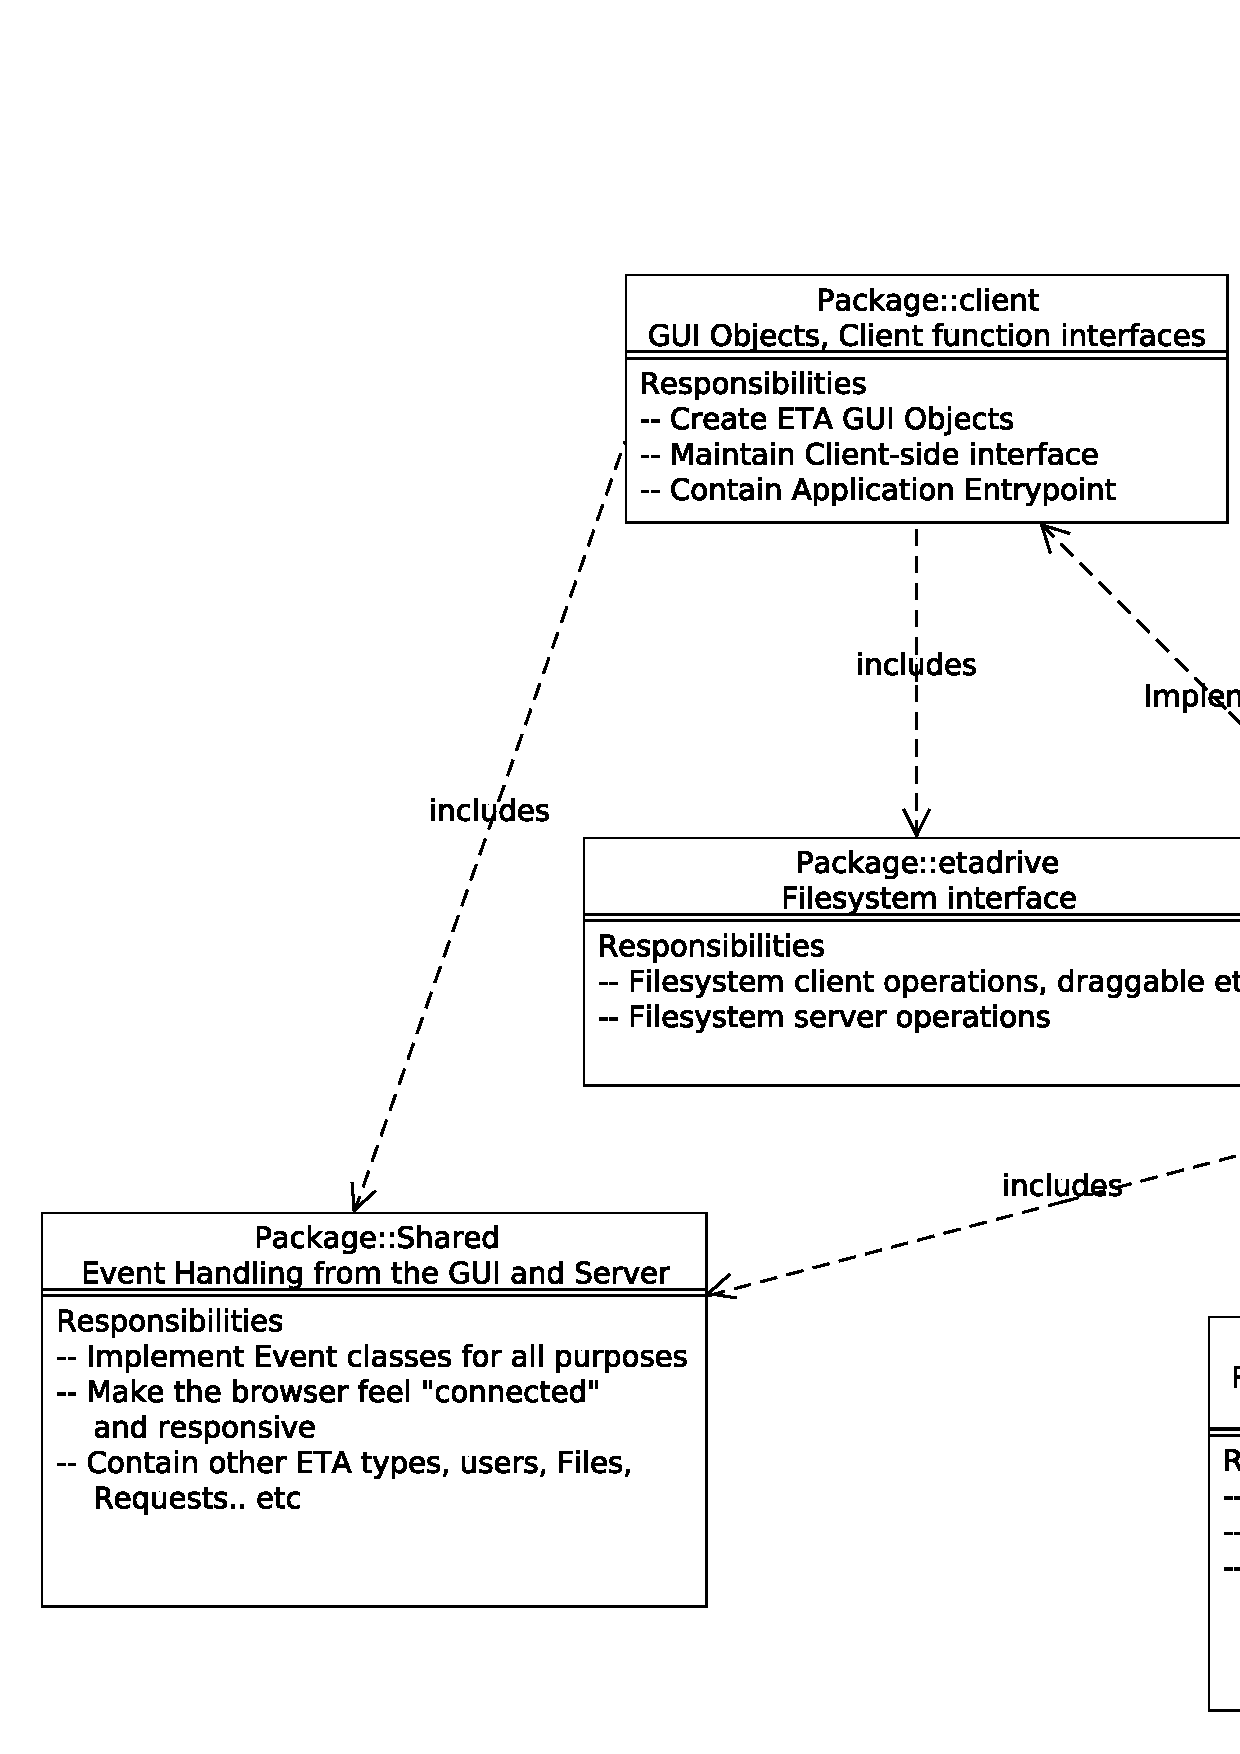
\includegraphics[width=1\textwidth]{ETAPackageOverview.jpg}
\caption{UML Diagram: ETA Package Overview}
\label{fig:ETAPackageOverview}
\end{figure}

\subsection{Dataflow}

 The way that ETA moves data is simple in concept, and complex in application. It is important to understand the different processes that belong to the Easy-Terminal-Alternative process group. These processes are, ETAStart, ETAMon, ETASubmit, and ETAUtil. Additionally, there are system services which ETA interacts, this is an authentication mechanism, a user manager, and a batch queue  for running jobs.
 
 When a user initially logs on, it first reaches the homepage of the web application. This is a HTML file which lives on the tomcat server. When a user logs into ETA, the server calls the authentication module, which then logs the user into the machine and executes ETAStart as that user. ETAStart is responsible for all of the interaction between the server and the user. It executes system calls, manages files, and submits jobs (Boyd). ETAStart is a persistent process and will not terminate unless explicitly told. 
 
 ETASubmit is the executable responsible for actually submitting the jobs to the batch system. ETASubmit is called from ETAStart, which will then finally call the monitoring process, ETAMon.
 
 ETAMon gets executed as the user anytime a job is submitted, it tracks the current progress of the job and notifies ETAStart when a job is finished. So when a user submits a job, ETAStart will call ETASubmit, which will then create an instance of ETAMon, which will then handle that job from start to finish.

 \begin{figure}
\includegraphics[width=1\textwidth]{DataflowDiagram.png}
\caption{Dataflow Diagram}
\label{fig:Dataflow Diagram}
\end{figure}
 \subsubsection{Job Submission}
 When a user first logs in, a token is created for that user in the database. This token will be used for authentication until their session has expired (ETA Source code). Upon authorization, a user can do several things, the most common being submitting a job. When a job is submitted, ETAStart executes the appropriate processes. An appropriate index is entered into the database representing the job. As long as this entry is active, the system will know the job is still running. ETAMon will handle the change of this value, which will then propagate it's way back to the end-user.
 
 The physical job will be run through the Sun Grid Engine Batch Scheduler. This is the scheduling and load balancing application for the CGRB cluster. Users may set several options, including total memory usage, estimated running time, number of execution threads, or even request a specific node to execute the job (Grid Entry Man Pages). Upon completion, the user will be notified and the standard output of the program will be displayed to the user. This information is stored in the users home directory under the folder ETA (ETA Source code). 

\subsubsection{Wrappers}
 The primary feature of Easy-Terminal-Alternative is to create wrappers, that is, web-driven forms that allow a user to interact with command line programs. When a user creates a wrapper, they choose a program from a list which is populated by ETAUtil. ETAUtil queries the server for a list of available applications (typically from the Linux /usr/bin folders). A user then inputs various fields which represent the different flags that are passed to the program. Upon completion, the wrapper is saved to the MySQL database.

 Each wrapper is associated with a user. These wrappers are typically private, but if marked as public (again stored in the database), any user may see and use the wrapper. When a job is submitted to ETASubmit, the command line arguments are parsed from the form built by the wrapper, and finally are placed into a string which will be submitted the Sun Grid Engine Batch scheduler.

\subsection{Runtime Environment}
Easy-Terminal-Alternative was designed to run on CentOS 6, and for the CGRB it is no different. Additionally, it requires a Batch scheduler, in this case The Sun Grid Engine. 

\section{Installation}

 Installing ETA is a non-trivial task. You need to know a few things about the architecture you are working on. These being, authentication mechanism and job scheduler. For the CGRB, these are NIS and Sun Grid Engine. These instructions are very technical and require a good understanding of Linux administration.
\subsection{Installing Dependencies}
 The first thing that must be done to install ETA is install the dependencies. These are, Java 7, the Apache Tomcat6 webserver, and the MySQL database engine. The Center for Genome Research and Biocomputing uses CentOS, so the package manager yum can be used to install them. Additionally, you will need to download the Google Web Toolkit compiler appropriate to the version of Java 7 that was downloaded.
\subsection{Downloading the source}
 To continue you need to download the source code, this can be done at https://github.com/cgrb/Easy-Terminal-Alternative. Once the files are downloaded, configure the install.sh script to point to your Java executable and your Google web toolkit executable. You will also need to create an ETA database in MySQL. To do this, you should run the eta\_ structure.sql file to build the structure (ETA Source Code).

\subsection{Configuring and building the source}

 The next thing that needs to be done is configure the files. There is a settings file in the war/WEB\- INF file which contains numerous settings. The file provided with the source is here:
 
 \lstinputlisting{settings}

 Most settings can be left blank, however the important ones are localpath, sqluser, sqluserpass, and sqlschemata. The first should point to where your service executables will live (see section 2.3), and the second should be the username, password, and database you configured for MySQL. It is vital that you do not let this file be world readable, as it contains sensitive information (Boyd).
 
 After configuring ETA, it must be built. Run the install.sh script you configured earlier. Then copy the outputted .jar files into the directory pointed to by localpath in the settings folder. Each of these files needs an associated shell script to execute them with the Java virtual machine.
 
\$JAVAHOME -jar
 \$ETASTART (Java Platform SE 7) is the command that should be used. JAVAHOME and ETASERVICE are environment variables that point to your java executable and to your ETA.jar file (One for each service). Next copy the war folder into your Tomcat apps folder. That is: /var/lib/tomcat6/webapps/ROOT/WEB\_ INF. Additionally, each of the .html and .js files from the source war folder need to be placed in /var/lib/tomcat6/webapps/ROOT/. Lastly, you must compile the C program spawnuser.c. This can be compiled with any standard C compiler and it's executable will need to be located in the localpath folder.
 
\subsection{Launching the application}

 To finally run ETA, you will need to start the tomcat service, and then navigate the Tomcat URL. If everything is working correctly you should be able to login as any user on the architecture and begin submitting jobs.


\section{Extension and Formal Documentation}
 Although ETA is perfectly configured for the Center for Genome Research and Biocomputing as it is, this does not mean the environment may change. This also applies for any other place that is running the software. This section will go over how to add a new module to ETA. Services are defined as unique Interfaces and Abstract classes. These are essentially contracts that require the child classes to implement these methods, this way, the rest of the application can be written referring to the service (knowing the methods exist), without worrying about how they are implemented (Java Platform SE 7).
\subsection{Services}
 Services is where most of the extension will be done. They are typically platform dependent and may need to be changed at any given time. The main services in ETA are the UserManager service, the RemoteUserManager service, and the Authentication service. All of these are dependent on the environment ETA is running on and may need to be implemented accordingly. To do so, all that must be done is implement the methods defined in the abstract classes.
 The service which does the most work is RemoteUserService. It is responsible for almost all of the interaction between the user and the server. The current implementation is ETAStart, which as said previously, is the service which get's executed any time a user logs in to ETA.
 

\section{Conclusion}
 Easy-Terminal-Alternative is a great solution to an ongoing problem. Researchers are able to bridge the technological gap much more easily, and computational people are allowed to spend more time developing new tools.
 
\subsection{Future work}
 ETA still is only configured for a few different environments. Adding new modules and modularizing more system dependent code will be a big step towards a complete package. Additionally, some kind of automated installer may be needed to allow for quick distribution. 


\setlength{\parindent}{0.5in}

\begin{workscited}

  \bibent
 Ambra Molesini, Alessandro Garcia, Christina von Flach Garcia Chavez, Thais Vasconcelos Batista, Stability assessment of aspect-oriented software architectures: A quantitative study, Journal of Systems and Software, Volume 83, Issue 5, May 2010, Pages 711-722, ISSN 0164-1212, 10.1016/j.jss.2009.05.022.
\\http://www.sciencedirect.com/science/article/pii/S0164121209001162. 

 \bibent
 "Apache Tomcat 6.0." \textit{Tomcat Documentation Index}. 9 Oct. 2012. Apache Foundation.  13 May 2013 http://tomcat.apache.org/tomcat-6.0-doc/. 
 
  \bibent
 Barbara Robbertse, Ryan J. Yoder, Alex Boyd, John Reeves, Joseph W. Spatafora. "Linux Bug \# 1: Bad Documentation". N.p., 7 Feb. 2011. Web. 30 May 2013.\\ 
http://www.ncbi.nlm.nih.gov/pmc/articles/PMC3038436/.

   \bibent
   Boyd, Alex. "Re: ETA Update" Message to the creator. 12 Dec. 2012. E-mail. An email with the original developer of Easy-Terminal-Alternative.
   
 \bibent
 Boyd, Alex. "Easy-Terminal-Alternative source code." Easy-Terminal-Alternative. Center for Genome Research and Biocomputing, 4, Sept. 2012. Web. 29, May 2013. 
\\https://www.github.com/cgrb/Easy-Terminal-Alternative. Source code to the actual application.

 \bibent
 "Google Web Toolkit." \textit{Developer's Guide}. 26 Oct. 2012. Google. 13 May 2013 \\https://developers.google.com/web-toolkit/doc/latest/DevGuide. 

 \bibent
 "Java Platform SE 7." \textit{Java Platform SE 7}. 28 July 2011. Oracle Inc. 13 May 2013 http://docs.oracle.com/javase/7/docs/api/. 


 \bibent
  Schroder, Carla. "Linux Bug \# 1: Bad Documentation" \textit{The Many Faces of Documentation}. N.p., 17 Nov. 2009. Web. 13 May 2013.\\ http://www.linuxplanet.com/linuxplanet/reports/6904/1/. 
  
   \bibent
   Sullivan, Chris. "Email Interview" Interview with Computational Scientist. 30 May. 2013. E-mail. An interview with the lead computational scientist at the Center for Genome Research and Biocomputing.
   
  \bibent
  "Sun Grid Engine." \textit{Man Pages}. Apr. 2008. Web. 28 May 2013. \\ http://gridscheduler.sourceforge.net/htmlman/manuals.html.
  
  
  







 \end{workscited}
 \newpage
 \section{Primary Sources}
 \subsection{Email with Alex Boyd (creator)}
.\\
ETA Update\\
Steve Hill hillst@onid.orst.edu\\
12/10/12\\
\\
I see you have compiled most of the class files into different .jar files, ETAMon, ETAStart, ETAMonitor, ETASubmit, ETAUtil...
\\
Where does tomcat need them to execute at?
\\
I noticed all your shell scripts as well that initialize everything. Do they all get run at once? Or does tomcat just execute the bash scripts on startup?
\\
What services execute ETAStart and ETA itself (I assume the latter is tomcat).
\\
When you apply an update, do you just pull the files from git and recompile them into their .jar files?
\\\\
Thanks again,
\\
Steve
\\\\\\
RE: ETA Update\\
Alex Boyd alex@cgrb.oregonstate.edu\\
12/14/12
 \\\\
Ah sorry, I haven't had time to respond. I will set you up with everything you need to test on waterman tomorrow (Saturday) 
\\
ETAStart is the service that spawns off as each user, ETA will issue an su command and than spawn and detach itself from the proccess. THis is done when a user logins\\
ETAMon gets run everytime a job runs and tells ETA that it started/stopped etc\\
ETASubmit is a command line utitlty to submit jobs though ETA\\
ETAUtil is another comand line utility that will give you information about files like what program produced them etc..
\\\\
There is a settings file in WEB\-INF called settings that has all the settings for eta. one of them is ETA\_Path or something like that and it points to /local/cluster/ETA/dev and all the jar files are there as well as the .so library used for the login 
So I have a compile script that pulls the latest version from git and makes all the jars and compiles the webapp with GWT, this is actually done on a different server, I will give you more details tomorrow as well.

\subsection{Email Interview With Chris Sullivan}


Before ETA, what problems did researchers typically have with computational work?\\\\
- All new tool were at the command line and it would take a great deal of time to port a tool into a web interface. This reduced the number of people who did computational work from a lack of knowledge on how to work in that environment.\\\\


How did the researchers solve those problems?\\\\

- Generally labs would hired physicists and computational scientist with knowledge to work in that environment to process data and make new tools. The CGRB had also developed a web portal system using MASON/perl and mysql. This included a tool called the Personal Sequence Database for with there is a pub (http://www.biomedcentral.com/1471-2105/8/479). The system was clunky and we needed to write a new page for every tool we wanted to have on the website.\\\\


What inspired the development and implementation of ETA?\\\\
- A tool called HAL (http://www.ncbi.nlm.nih.gov/pmc/articles/PMC3038436/) made in the Spatafora lab needed a web portal system to allow more users to interact with the tool. Alex Boyd created a tool to start this process and once I talked with him about it we both realized it could be expanded into the tool we call ETA today. My past knowledge of problems with programming tools onto the web and methods to interact with the cluster help drive the path we took and why the system works the way it does (ie wrappers, pipelines, requests...).
\\\\

What were the goals for ETA?\\\\
- Allow any user on the system to create new web driven forms to any command line tool in minutes/hours versus days/weeks. Then take these wrappers and share them to other users and combine them together into pipelines. Next we wanted to allow the computational people to focus on writing new tools versus just processing data which can be done by other lab members is provided the proper means. To this end a computational person can create new wrappers and pipelines to any command line tool as well as tools personally created and share them to other specific users on the system or to the public. Finally we need a method to upload, download and disseminate data using the interface.
\\\\

Are there any future plans for ETA? If so what are they?\\\\

- yeah we need to make a pub for it right away!\\\\

\end{document}